\achapter{9}{Introduction to Eigenvalues and Eigenvectors} \label{chap:intro_eigenvals_eigenvects}

\vspace*{-17 pt}
\framebox{
\parbox{\dimexpr\linewidth-3\fboxsep-3\fboxrule}
{\begin{fqs}
\item What is an eigenvalue of a matrix?
\item What is an eigenvector of a matrix?
\item How do we find eigenvectors of a matrix corresponding to an eigenvalue?
\item How can the action of a matrix on an eigenvector be visualized?
\item Why do we study eigenvalues and eigenvectors?
\item What are discrete dynamical systems and how do we analyze the long-term behavior in them?
\end{fqs}}}% \hspace*{3 pt}}

\vspace*{13 pt}

\csection{Application: The Google PageRank Algorithm}
\label{sec:appl_pagerank}
The World Wide Web is a vast collection of information, searchable via search engines. A search engine looks for pages that are of interest to the user. In order to be effective, a search engine needs to be able to identify those pages that are relevant to the search criteria provided by the user. This involves determining the relative importance of different web pages by ranking the results of thousands or millions of pages fitting the search criteria. For Google, the PageRank algorithm is their method and is ``the heart of our software'' as they say. It is this PageRank algorithm that we will learn about later in this section. Eigenvalues and eigenvectors play an important role in this algorithm.

\csection{Introduction}
\label{sec:eigen_intro}

Given a matrix $A$, for some special non-zero vectors $\vv$ the action of $A$ on $\vv$ will be same as scalar multiplication, i.e., $A\vv=\lambda \vv$ for some scalar $\lambda$. Geometrically, this means that the transformation $T$ defined by $T(\vx) = A\vx$ simply stretches or contracts the vector $\vv$ but does not change its direction. Such a \underline{nonzero} vector is called an \emph{eigenvector} of $A$, while the scalar $\lambda$ is called the corresponding \emph{eigenvalue} of $A$. The eigenvectors of a matrix tell us quite a bit about the transformation the matrix defines. 

Eigenvalues and eigenvectors are used in many applications. Social media like Facebook and Google use eigenvalues to determine the influence of individual members on the network (which can affect advertising) or to rank the importance of web pages. Eigenvalues and eigenvectors appear in quantum physics, where atomic and molecular orbitals can be defined by the eigenvectors of a certain operator. They appear in principal component analysis, used to study large data sets, to diagonalize certain matrices and determine the long term behavior of systems as a result, and in the important singular value decomposition of a matrix. Matrices with real entries can have real or complex eigenvalues, and complex eigenvalues reveal a rotation that is encoded in every real matrix with complex eigenvalues which allows us to better understand certain matrix transformations. 

\begin{definition} \label{def:eigenvector} Let $A$ be an $n \times n$ matrix. A non-zero vector $\vx$ is an \textbf{eigenvector}\index{eigenvector} (or \textbf{characteristic vector}\index{characteristic vector}) of $A$ if there is a scalar $\lambda$ such that
$A\vx = \lambda \vx$.
The scalar $\lambda$ is an \textbf{eigenvalue}\index{eigenvalue} (or \textbf{characteristic value}\index{characteristic value}) of $A$.
\end{definition}

For example, $\vv= \left[ \begin{array}{c} 1\\1\end{array} \right]$ is an eigenvector of $A=\left[ \begin{array}{cc} 2 & 1 \\ 3 & 0 \end{array} \right]$ corresponding to the eigenvalue $\lambda=3$ because $A\vv = \left[ \begin{array}{c} 3\\3\end{array} \right]$, which is equal to $3\vv$. On the other hand, $\vw= \left[ \begin{array}{c} 1\\2\end{array} \right]$ is not an eigenvector of $A=\left[ \begin{array}{cc} 2 & 1 \\ 3 & 0 \end{array} \right]$ because $A\vw = \left[ \begin{array}{c} 4\\3\end{array} \right]$, which is not a multiple of $\vw$.



\begin{pa} \label{pa:2_b_1} ~
\be
\item For each of the following parts, use the definition of an eigenvector to determine whether the given vector $\vv$ is an eigenvector for the given matrix $A$. If it is, determine the corresponding eigenvalue. 

\ba
\item $A=\left[ \begin{array}{cc} 3 &2 \\ 3 & 8 \end{array} \right]$, $\vv=\left[ \begin{array}{r} -2\\1 \end{array} \right]$

\item $A=\left[ \begin{array}{cr} 2 & 0 \\ 0 & -3 \end{array} \right]$, $\vv=\left[ \begin{array}{c} 0\\1 \end{array} \right]$

\item $A=\left[ \begin{array}{cc} 3 &2 \\ 3 & 8 \end{array} \right]$, $\vv=\left[ \begin{array}{c} 1\\1 \end{array} \right]$

\item $A=\left[ \begin{array}{cc} 1 &2 \\ 2 & 4 \end{array} \right]$, $\vv=\left[ \begin{array}{r} -2\\1 \end{array} \right]$ 

\ea

\item We now consider how we can find the eigenvectors corresponding to an eigenvalue using the definition. Suppose $A=\left[ \begin{array}{cr} 6 & -2\\2 & 1 \end{array} \right]$. We consider whether we can find eigenvectors corresponding to eigenvalues 3, and 5. Effectively, this will help us determine whether 3 and/or 5 are eigenvalues of $A$.

\ba
	\item Rewrite the vector equation $A\vv=5\vv$ where $\vv = \left[ \begin{array}{c} x \\y \end{array} \right]$ as a vector equation.
	
	
	\item After writing $5\vv$ as $5I\vv$ where $I$ is the identity matrix, rearrange the variables to turn this vector equation into the homogeneous matrix equation $B\vv=\vzero$ where $B=\left[ \begin{array}{cr} 1 & -2\\2 & -4 \end{array} \right]$. If possible, find a non-zero (i.e. a non-trivial) solution to $B\vv=\vzero$. Explain what this means about 5 being an eigenvalue of $A$ or not. 


\item Similarly, determine whether the vector equation $A\vv=3\vv$ has non-zero solutions. Using your result, determine whether 3 is an eigenvalue of $A$ or not.

\ea

\ee
\end{pa}


\csection{Eigenvalues and Eigenvectors}

Eigenvectors are especially useful in understanding the long-term behavior of dynamical systems, an example of which we will see shortly. The long-term behavior of a dynamical system is quite simple when the initial state vector is an eigenvector and this fact helps us analyze the system in general. 

To find eigenvectors, we are interested in determining the vectors $\vx$ for which $A\vx$ has the same direction as $\vx$. This will happen when
\[A\vx = \lambda \vx\]
for some scalar $\lambda$. Of course, $A\vx = \lambda \vx$ when $\vx = \vzero$ for every $A$ and every $\lambda$, but that is uninteresting. So we really want to consider when there is a \underline{non-zero} vector $\vx$ so that $A\vx = \lambda \vx$. This prompts the definition of eigenvectors and eigenvalues as in Definition \ref{def:eigenvector} 


In order for a matrix $A$ to have an eigenvector, one condition $A$ must satisfy is that $A$ has to be a square matrix\index{matrix!square}, i.e. an $n \times n$ matrix. We will find that each $n\times n$ matrix has only finitely many eigenvalues.

The terms eigenvalue and eigenvector seem to come from Hilbert, using the German ``eigen'' (roughly translated as ``own'', ``proper'', or ``characteristic'') to emphasize how eigenvectors and eigenvalues are connected to their matrices. To find the eigenvalues and eigenvectors of an $n \times n$ matrix $A$, we need to find the solutions to the equation
\[A \vx = \lambda \vx \, .\]
In Preview Activity \ref{pa:2_b_1}, we considered this equation for $A=\left[ \begin{array}{cr} 6&-2 \\ 2&1 \end{array} \right]$ and $\lambda=5$. The homogeneous matrix equation we came up with was
\[ \left[ \begin{array}{cr} 1&-2 \\ 2&-4 \end{array}\right] \vx = \vzero \,.\]
To see the relationship between this homogeneous matrix equation and the eigenvalue-eigenvector equation better, let us consider the eigenvector equation using matrix algebra:
\begin{align*}
A\vx &= \lambda\vx \\
A\vx - \lambda \vx &= \vzero \\
A\vx - \lambda I_n\vx &= \vzero \\
(A-\lambda I_n)\vx &= \vzero,
\end{align*}
where $I_n$ is the $n \times n$ identity matrix. Notice that this description matches the homogenous equation matrix example above since we simply subtracted 5 from the diagonal terms of the matrix $A$. Hence, to find eigenvalues, we need to find the values of $\lambda$ so that the homogeneous equation $(A - \lambda I_n)\vx=\vzero$ has non-trivial solutions.



\begin{activity} \hfill
\ba
\item Under what conditions on $A-\lambda I_n$ will the matrix equation $(A-\lambda I_n)\vx=\vzero$ have non-trivial solutions? Describe at least two different but equivalent conditions. 



\item The real number 0 is an eigenvalue of $A = \left[ \begin{array}{cc} 1&2 \\ 2&4 \end{array} \right]$. Check that your criteria in the previous part agrees with this result.



\item Determine if 5 is an eigenvalue of the matrix $A = \left[ \begin{array}{cc} 1&2 \\ 2&4 \end{array} \right]$ using your criterion above. 

 

%\item (If time: Just for fun) Which $A = \left[ \begin{array}{cc} a&b\\c&d \end{array} \right]$ matrices have $ \left[ \begin{array}{c} 1\\ 1 \end{array} \right]$ as an eigenvector? More generally, for which $n\times n$ matrices is the vector with all 1's an eigenvector?
%
%

%\item What is the other eigenvalue of $A = \left[ \begin{array}{cc} 1&2\\2&4 \end{array} \right]$?



\item What are the two eigenvalues of the matrix $A = \left[ \begin{array}{cc} 3&2\\4&5 \end{array} \right]$?



\ea

\end{activity}



Since an eigenvector of $A$ corresponding to eigenvalue $\lambda$ is a non-trivial solution to the homogeneous equation $(A - \lambda I_n)\vx = \vzero$, the eigenvalues $\lambda$ which work are those for which the matrix $A-\lambda I_n$ has linearly dependent columns, or for which the row echelon form of the matrix $A-\lambda I_n$ does not have a pivot in every column. When we need to test if a specific $\lambda$ is an eigenvalue, this method works fine. However, finding which $\lambda$'s will work in general involves row reducing a matrix with $\lambda$'s subtracted on the diagonal algebraically. For certain types of matrices, this method still provides us the eigenvalues quickly. For general matrices though, row reducing algebraically is not efficient. We will later see an algebraic method which uses the determinants to find the eigenvalues.



\begin{activity} ~
\ba
\item For $\lambda$ to be an eigenvalue of $A$, we noted that $A-\lambda I_n$ must have a non-pivot column. Use this criterion to explain why $A=\left[ \begin{array}{rc} -2&2\\0&4 \end{array} \right]$ has eigenvalues $\lambda=-2$ and $\lambda=4$.



\item Determine the eigenvalues of $A = \left[ \begin{array}{ccrc} 3&0&1&0 \\ 0&2&-1&0 \\ 0&0&2&0 \\ 0&0&0&1 \end{array} \right]$. 



\item Generalize your results from the above parts in the form of a theorem in the most general $n\times n$ case.



\ea
\end{activity}

\csection{Dynamical Systems}
\label{sec:dynam_sys}

One real-life application of eigenvalues and eigenvectors is in analyzing the long-term behavior of \emph{discrete dynamical systems}. A \emph{dynamical system}\index{dynamical system} is a system of variables whose values change with time. In discrete systems, the change is described by defining the values of the variables at time $t+1$ in terms of the values at time $t$. For example, the discrete dynamical system 
\[y_{t+1} = y_t + t\]
relates the value of $y$ at time $t+1$ to the value of $y$ at time $t$. This is in contrast with a differential equation\footnote{A differential equation is an equation that involves one or more derivatives of a function.}  such as  
\[ \frac{dy}{dt} = y+t,\]
which describes the instantaneous rate of change of $y(t)$ in terms of $y$ and $t$.

Discrete dynamical systems can be used in population modeling to provide a simplified model of predator-prey interactions in biology (see Preview Activity \ref{pa:2_b_2}). Other applications include Markov chains (see Exercise \ref{ex:2_b_Markov}), age structured population growth models, distillation of a binary ideal mixture of two liquids, cobweb model in economics concerning the interaction of supply and demand for a single good, queuing theory and traffic flow. 

Eigenvectors can be used to analyze the long-term behavior of dynamical systems.

\begin{pa} \label{pa:2_b_2} ~
\be
\item Consider a discrete dynamical system providing a simplified model of predator-prey interactions in biology, such as the system describing the populations of rabbits and foxes in a certain area. 

Suppose, for example, for a specific area the model is given by the following equations:
%\begin{equation} \label{eq:PA5.1_3}
%\begin{array} {rcl}
%r_{k+1}&=&1.14 r_k - 0.12 f_k\\ 
%f_{k+1}&=&0.08 r_k +0.86 f_k
%\end{array}
%\end{equation}
\begin{equation}  \label{eq:PA5.1_3}
\begin{alignedat}{4}
r_{k+1}	&{}={} 	&{1.14}r_k 	&{}-{}	&{0.12}f_k \\
f_{k+1}	&{}={} 	&{0.08}r_k 	&{}+{}	&{0.86}f_k \\
\end{alignedat}
\end{equation}
where $r_i$ represents the number of rabbits in the area $i$ years after a starting time value, and $f_i$ represents the number of foxes in year $i$. We use $r_0, f_0$ to denote the initial population values.

\ba
\item Suppose $r_k=300$ and $f_k=100$ for one year. Calculate rabbit and fox population values for the next year. In other words, find $r_{k+1}, f_{k+1}$ values.

\item Consider the coefficients of the variables $r_k, f_k$ in the the system of equations in (\ref{eq:PA5.1_3}). Can you explain the reasoning behind the signs and absolute sizes of the coefficients from the story that it models? 

\item Let $\vx_k=\left[ \begin{array}{c} r_k \\ f_k \end{array} \right]$. The vector $\vx_k$ is called the \emph{state vector} of the system at time $k$, because it describes the state of the whole system at time $k$. We can rewrite the system of equations in (\ref{eq:PA5.1_3}) as a matrix-vector equation in terms of the state vectors at time $k$ and $k+1$. More specifically, the equation will be of the form 
\begin{equation} \label{eq:PA5.1_4}
\vx_{k+1} = A\vx_k
\end{equation}
where $A = \left[ \begin{array}{cr} 1.14 & -0.12 \\ 0.08 & 0.86 \end{array} \right]$. We will call this matrix the \emph{transition matrix} of the system. Check that $A \left[ \begin{array}{c} 300\\100 \end{array} \right]$ gives us the population values you calculated in the first part above.

\item The transition matrix will help us simplify calculations of the population values. Note that equation (\ref{eq:PA5.1_4}) implies that $\vx_1 = A\vx_0$, $\vx_2=A\vx_1$, $\vx_3=A\vx_2$, and so on. This is a recursive method to find the population values as each year's population values depend on the previous year's population values. Using this approach, calculate $\vx_k$ for $k$ values up to 5 corresponding to the following \underline{three different} initial rabbit-fox population values (all in thousands): 
\[ r_0=300 \;,\;  f_0=100 \]
\[ r_0=100 \;,\;  f_0=200 \]
\[ r_0=1200 \;,\; f_0=750\]
Can you guess the long-term behavior of the population values in each case? Are they both increasing? Decreasing? One increasing, one decreasing? How do the rabbit and fox populations compare?

	\ea


\ee
\end{pa}


A dynamical system is a system of variables whose values change with time. In Preview Activity \ref{pa:2_b_2}, we considered the discrete dynamical system modeling the rabbit and fox population in an area, which is an example of a predator-prey system. The system was given by the equations from (\ref{eq:PA5.1_3}), where $r_i$ represented the number of rabbits in the area $i$ years after a starting time value, and $f_i$ represented the number of foxes in year $i$. In this notation, $r_0, f_0$ corresponded to the initial population values.

As we saw in Preview Activity \ref{pa:2_b_2}, if we define the state vector\index{state vector} as $\vx_k=\begin{bmatrix} r_k \\ f_k \end{bmatrix}$, the system of equations representing the dynamical system can be expressed as  
\begin{equation} 
\vx_{k+1} = A \vx_k \label{eq:state_vector_recursive_formula}
\end{equation}
where $A=\left[ \begin{array}{cr} 1.14 & -0.12 \\ 0.08 & 0.86 \end{array} \right]$ represents the transition matrix. Note that equation (\ref{eq:state_vector_recursive_formula}) encodes infinitely many equations including $\vx_1 = A\vx_0$, $\vx_2=A\vx_1$, $\vx_3=A\vx_2$, and so on. This is a recursive formula for the population values as each year's population values are expressed in terms of the previous year's population values. If we want to calculate $\vx_{10}$, this formula requires first finding the population values for years 1-9. However, we can obtain a non-recursive formula using matrix algebra. If we substitute $\vx_1 = A\vx_0$ into $\vx_2=A\vx_1$ and simplify, we find that 
\[ \vx_2=A\vx_1= A(A\vx_0) = A^2 \vx_0 \,.\] 
Similarly, substituting $\vx_2=A^2\vx_1$ into the formula for $\vx_3$ gives
\[ \vx_3 = A\vx_2=A(A^2 \vx_0) = A^3 \vx_0 \, .\]
This process can be continued inductively to show that 
\begin{equation}
\vx_k=A^k \vx_0 \label{eq:state_vector_closed_formula}
\end{equation}
for every $k$ value. So to find the population values at any year $k$, we only need to know the initial state vector $\vx_0$.



\begin{activity} \label{act:dynamical_system} In this activity the matrix $A$ is the transition matrix for the rabbit and fox population model,
\[A = \left[ \begin{array}{cr} 1.14 & -0.12 \\ 0.08 & 0.86 \end{array} \right].\]
\ba
\item Suppose that the initial state vector $\vx_0$ is an eigenvector of $A$ corresponding to eigenvalue $\lambda$. In this case, explain why $\vx_1=\lambda \vx_0$ and $\vx_2=\lambda^2 \vx_0$. Find the formula for $\vx_k$ in terms of $\lambda, k$ and $\vx_0$ by applying equation (\ref{eq:state_vector_recursive_formula}) iteratively.



\item The initial state vector $\vx_0=\left[ \begin{array}{c} 300\\100\end{array} \right]$ is an eigenvector of $A$. Find the corresponding eigenvalue and, using your formula from (a) for $\vx_k$ in terms of $\lambda, k$ and $\vx_0$, find the state vector $\vx_k$ in this case.



\item The initial state vector $\vx_0=\left[ \begin{array}{c} 100\\200 \end{array} \right]$ is an eigenvector of $A$. Find the corresponding eigenvalue and, using your formula from (a) for $\vx_k$ in terms of $\lambda, k$ and $\vx_0$, find the state vector $\vx_k$ in this case.



\item Consider now an initial state vector of the form $\vx_0=a\vv_0+b\vw_0$ where $a, b$ are constants, $\vv_0$ is an eigenvector corresponding to eigenvalue $\lambda_1$ and $\vw_0$ corresponding to eigenvalue $\lambda_2$ ($\vv_0$ and $\vw_0$ are not necessarily the eigenvectors from parts (b) and (c)). Use matrix algebra and equation (\ref{eq:state_vector_closed_formula}) to explain why $\vx_k=a\lambda_1^k\vv_0+b\lambda_2^k\vw_0$.



\item Express the initial state vector $\vx_0=\left[ \begin{array}{c} 1200 \\ 750 \end{array} \right]$ as a linear combination of the eigenvectors $\vv_0=\left[ \begin{array}{c}300\\ 100\end{array} \right], \vw_0=\left[ \begin{array}{c} 100\\200\end{array} \right]$ and use your result from the previous part to find a formula for $\vx_k$. What happens to the population values as $k\to \infty?$


\ea

\end{activity}

As you discovered in Activity \ref{act:dynamical_system}, we can use linearly independent eigenvectors of the transition matrix to find a closed formula for the state vector of a dynamical system, as long as the initial state vector can be expressed as a linear combination of the eigenvectors.


\csection{Examples}
\label{sec:eigen_exam}

\ExampleIntro

\begin{example} Let $A = \left[ \begin{array}{cc} 1&2\\2&4 \end{array} \right]$.
	\ba
	\item Find all of the eigenvalues of $A$.
	
	\item Find a corresponding eigenvector for each eigenvalue found in part (a).  
	
	\ea


\ExampleSolution
\ba

\item Recall that a scalar $\lambda$ is a eigenvalue for $A$ if there is a nonzero vector $\vx$ such that $A \vx = \lambda \vx$ or $(A-\lambda I_2) \vx = \vzero$. For this matrix $A$, we have 
\[A - \lambda I_2 = \left[ \begin{array}{cc} 1-\lambda&2\\2&4-\lambda \end{array} \right].\]
To solve the homogeneous system $(A-\lambda I_2) \vx = \vzero$, we row reduce $A - \lambda I_2$. To do this, we first interchange rows to get the following matrix that is row equivalent to $A - \lambda I_2$ (we do this to ensure that we have a nonzero entry in the first row and column)
\[\left[ \begin{array}{cc} 2&4-\lambda \\ 1-\lambda&2 \end{array} \right].\]
Next we replace row two with $\frac{1}{2}(1-\lambda)$ times row one minus row two to obtain the row equivalent matrix
\[\left[ \renewcommand{\arraystretch}{1.4} \begin{array}{cc} 2&4-\lambda \\ 0&\frac{1}{2}(4-\lambda)(1-\lambda)-2 \\ \end{array} \right].\]
There will be a nontrivial solution to $(A-\lambda I_2)\vx = \vzero$ if there is a row of zeros in this row echelon form. Thus, we look for values of $\lambda$ that make 
\[\frac{1}{2}(4-\lambda)(1-\lambda)-2 = 0.\]
Applying a little algebra shows that 
\begin{align*}
\frac{1}{2}(4-\lambda)(1-\lambda)-2 &= 0 \\
(4-\lambda)(1-\lambda) - 4 &= 0 \\
\lambda^2 - 5 \lambda &= 0 \\
\lambda(\lambda-5) &= 0.
\end{align*}
So the eigenvalues of $A$ are $\lambda = 0$ and $\lambda = 5$. 

\item Recall that an eigenvector for the eigenvalue $\lambda$ is a nonzero vector $\vx$ such that $(A - \lambda I_2) \vx = \vzero$. We consider each eigenvalue in turn. 
\begin{itemize}
\item When $\lambda = 0$, 
\[A - 0 I_2 = A = \left[ \begin{array}{cc} 1&2\\2&4 \end{array} \right].\]
Technology shows that the reduced row echelon form of $A$ is 
\[\left[ \begin{array}{cc} 1&2 \\ 0&0 \end{array} \right].\]
If $\vx = \left[ \begin{array}{c} x_1\\x_2 \end{array} \right]$, then $A \vx = \vzero$ implies that $x_2$ is free and $x_1 = -2x_2$. Choosing $x_2 = 1$ gives us the eigenvector $\left[ \begin{array}{r} -2\\1 \end{array} \right]$. As a check, note that 
\[\left[ \begin{array}{cc} 1&2\\2&4 \end{array} \right] \left[ \begin{array}{r} -2\\1 \end{array} \right] = \left[ \begin{array}{c} 0\\0 \end{array} \right].\]

\item When $\lambda = 5$, 
\[A - 5 I_2 = \left[ \begin{array}{rr} -4&2\\2&-1 \end{array} \right].\]
Technology shows that the reduced row echelon form of $A-5I_2$ is 
\[\left[ \renewcommand{\arraystretch}{1.4} \begin{array}{cr} 1&-\frac{1}{2} \\ 0&0 \end{array} \right].\]
If $\vx = \left[ \begin{array}{c} x_1\\x_2 \end{array} \right]$, then $(A - 5I_2)\vx = \vzero$ implies that $x_2$ is free and $x_1 = \frac{1}{2}x_2$. Choosing $x_2 = 2$ gives us the eigenvector $\left[ \begin{array}{c} 1\\2 \end{array} \right]$. As a check, note that 
\[\left[ \renewcommand{\arraystretch}{1.4} \begin{array}{cr} 1&-\frac{1}{2} \\ 0&0 \end{array} \right] \left[ \begin{array}{c} 1\\2 \end{array} \right] = \left[ \begin{array}{c} 0\\0 \end{array} \right].\]

\end{itemize}
\ea

\end{example}
 
\begin{example} Accurately predicting the weather has long been an important task. Meteorologists  use science, mathematics, and technology to construct models that help us understand weather patterns. These models are very sophisticated, but we will consider only a simple model. Suppose, for example, we want to learn something about whether it will be wet or dry in Grand Rapids, Michigan. To do this, we might begin by collecting some data about weather conditions in Grand Rapids and then use that to make predictions. Information taken over the course of 2017 from the National Weather Service Climate Data shows that if it was dry (meaning no measurable precipitation, either rain or snow) on a given day in Grand Rapids, it would be dry the next day with a probability of 64\% and wet with a probability of 36\%. Similarly, if it was wet on a given day it would be dry the next day with a probability of 47\% and dry with a probability of 53\%. Assuming that this pattern is one that continues in the long run, we can develop a mathematical model to make predictions about the weather. 

This data tells us how the weather transitions from one day to the next, and we can succinctly represent this data in a \emph{transition matrix}\index{transition matrix}:
\begin{equation} \label{eq:weather_transition}
T = \left[ \begin{array}{cc} 0.64&0.47 \\ 0.36&0.53 \end{array} \right].
\end{equation}
Whether it is dry or wet on a given day is called the \emph{state} of that day. So our transition matrix tells us about the transition between states. Notice that if $T = [t_{ij}]$, then the probability of moving from state $j$ to state $i$ is given by $t_{ij}$. We can represent a state by a vector: the vector $\left[ \begin{array}{c} 1\\0 \end{array}\right]$ represents the dry state and the vector $\left[ \begin{array}{c} 0\\1 \end{array}\right]$ represents the wet state. 

	\ba
	\item Calculate $T\left[ \begin{array}{c} 1\\0 \end{array}\right] $. Interpret the meaning of this output.
	

	\item Calculate $T\left[ \begin{array}{c} 0\\1 \end{array}\right] $. Interpret the meaning of this output.
	

	\item Calculate $T\left[ \begin{array}{c} 0.3\\0.7 \end{array}\right] $. Interpret the meaning of this output.


	\item We can use the transition matrix to build a chain of probability vectors. We begin with an initial state, say it is dry on a given day. This initial state is represented by the initial state vector $\vx_0 = \left[ \begin{array}{c} 1\\0 \end{array}\right]$. The probabilities that it will be dry or wet the following day are given by the vector 
\[\vx_1 = T\vx_0 = \left[ \begin{array}{c} 0.64\\0.36 \end{array}\right].\]
This output vector tells us that the next day will be dry with a 64\% probability and wet with a 36\% probability. 

For each $k \geq 1$, we let 
\begin{equation} \label{eq:weather_chain}
\vx_{k} = T\vx_{k-1}.
\end{equation}
Thus we create a sequence of vectors that tell us the probabilities of it being dry or wet on subsequent days. The vector $\vx_k$ is called the \emph{state vector} of the system at time $k$, because it describes the state of the whole system at time $k$. We can rewrite the system of equations in (\ref{eq:PA5.1_3}) as a matrix-vector equation in terms of the state vectors at time $k$ and $k+1$. More specifically, the equation will be of the form 
\begin{equation} \label{eq:weather_chain}
\vx_{k+1} = T\vx_k
\end{equation}
for $k \geq 0$. 
	\begin{enumerate}[i.]
	\item Starting with $\vx_0 = \left[ \begin{array}{c} 1\\0 \end{array} \right]$, use appropriate technology to  calculate $\vx_k$ for $k$ values up to 10. Round to three decimal places. What do you notice about the entries? 
	
	\item What does the result of the previous part tell us about eigenvalues of $T$? Explain. 
	
	\item Rewrite $T$ as 
	\[T = \left[ \renewcommand{\arraystretch}{1.4} \begin{array}{cc} \frac{64}{100}&\frac{47}{100} \\ \frac{36}{100}&\frac{53}{100} \end{array} \right].\]
	 We do this so we can use exact arithmetic. Let $\vx = \left[ \renewcommand{\arraystretch}{1.4} \begin{array}{c} \frac{47}{83} \\ \frac{36}{83} \end{array} \right]$. What is $T\vx$? (Use exact arithmetic, no decimals.) Explain how $\vx$ is related to the previous two parts of this problem. What does the vector $\vx$ tells us about weather in Grand Rapids? 
	
	\end{enumerate}


\ea
	
\ExampleSolution
\ba
\item Here we have 
\[T\left[ \begin{array}{c} 1\\0 \end{array}\right]  = \left[ \begin{array}{cc} 0.64&0.47 \\ 0.36&0.53 \end{array} \right] \left[ \begin{array}{c} 1\\0 \end{array}\right]  = \left[ \begin{array}{c} 0.64\\0.36 \end{array}\right].\]
This output tells us the different probabilities of whether it will be dry or wet the day following a dry day. 



\item Here we have 
\[T\left[ \begin{array}{c} 0\\1 \end{array}\right]  = \left[ \begin{array}{cc} 0.64&0.47 \\ 0.36&0.53 \end{array} \right] \left[ \begin{array}{c} 0\\1 \end{array}\right]  = \left[ \begin{array}{c} 0.47\\0.53 \end{array}\right].\]
This output tells us the different probabilities of whether it will be dry or wet the day following a wet day. 


	\item Here we have 
\[T\left[ \begin{array}{c} 0.3\\0.7 \end{array}\right]  = \left[ \begin{array}{cc} 0.64&0.47 \\ 0.36&0.53 \end{array} \right] \left[ \begin{array}{c} 0.3\\0.7 \end{array}\right]  \approx \left[ \begin{array}{c} 0.52\\0.48 \end{array}\right].\]
This output tells us there is a 52\% chance of it being dry and a 48\% chance of it being wet following a day when there is a 30\% chance of it being dry and a 70\% chance of it being wet. 

	\item 
	\begin{enumerate}[i.]
	\item Technology shows that
	\[
	\begin{array}{ll}
	\vx_1 = \left[ \begin{array}{c} 0.640\\0.360 \end{array} \right] &
	\vx_2 = \left[ \begin{array}{c} 0.579\\0.421 \end{array} \right] \vspace{2pt} \\
	\vx_3 = \left[ \begin{array}{c} 0.568\\0.432 \end{array} \right] &
	\vx_4 = \left[ \begin{array}{c} 0.567\\0.433 \end{array} \right]  \vspace{2pt}  \\
	\vx_5 = \left[ \begin{array}{c} 0.566\\0.434 \end{array} \right] &
	\vx_6 = \left[ \begin{array}{c} 0.566\\0.434 \end{array} \right]  \vspace{2pt}  \\
	\vx_7 = \left[ \begin{array}{c} 0.566\\0.434 \end{array} \right] &
	\vx_8 = \left[ \begin{array}{c} 0.566\\0.434 \end{array} \right]  \vspace{2pt}  \\
	\vx_9 = \left[ \begin{array}{c} 0.566\\0.434 \end{array} \right] &
	\vx_{10} = \left[ \begin{array}{c} 0.566\\0.434 \end{array} \right].
	\end{array} \]
	We can see that our vectors $\vx_k$ are essentially the same as we let $k$ increase. 
	
	\item Since our sequence seems to be converging to a vector $\vx$ satisfying $T \vx = \vx$, we conclude that 1 is an eigenvalue of $T$. 
	
	\item  A matrix vector multiplication shows that 
	\[T \vx = \left[ \renewcommand{\arraystretch}{1.4} \begin{array}{cc} \frac{64}{100}&\frac{47}{100} \\ \frac{36}{100}&\frac{53}{100} \end{array} \right]\left[ \renewcommand{\arraystretch}{1.4} \begin{array}{c} \frac{47}{83} \\ \frac{36}{83} \end{array} \right] = \left[ \renewcommand{\arraystretch}{1.4} \begin{array}{c} \frac{47}{83} \\ \frac{36}{83} \end{array} \right].\]
In other words, $\vx$ is an eigenvector for $T$ with eigenvalue 1. Notice that 
\[\frac{47}{83} \approx 0.566 \ \text{ and } \ \frac{36}{83} \approx 0.434,\]
so these fractions give the same results we obtained with our sequence of vectors $\vx_k$. These vectors provide a steady-state vector for Grand Rapids weather. In other words, if there is a $56.6\%$ chance of it being dry on a given day in Grand Rapids, then there is a $56.6\%$ chance it will be dry again the next day. 
	
	\end{enumerate}
	
\ea

This is an example of a Markov process\index{Markov process}. Markov processes (named after Andrei Andreevich Markov) are widely used to model phenomena in biology, chemistry, business, physics, engineering, the social sciences, and much more. More specifically, 

\begin{definition} \label{def:Markov}  A \textbf{Markov process}\index{Markov process} is a process in which the probability of the system being in a given state depends only on the previous state.
\end{definition}

If $\vx_0$ is a vector which represents the initial state of a Markov process, then there is a matrix $T$ (the \emph{transition matrix})\index{transition matrix} such that the state of the system after one iteration is given by the vector $T\vx_0$. This produces a chain of state vectors $T\vx_0$, $T^2 \vx_0$, $T^3 \vx_0$, etc., where the state of the system after $n$ iterations is given by $T^n \vx_0$.  Such a chain of vectors is called a \emph{Markov chain}\index{Markov chain}. A Markov process is characterized by two properties:
\begin{itemize}
\item the total number of observations remains fixed (this is reflected in the fact that the sum of the entries in each column of the matrix $T$ is 1), and
\item no observation is lost (this means the entries in the matrix $T$ cannot be negative).
\end{itemize}


\end{example}

\csection{Summary}
\label{sec:eigen_summ}
We learned about eigenvalues and eigenvectors of a matrix in this section.
\begin{itemize}
\item A scalar $\lambda$ is an  eigenvalue (or characteristic value) of a square matrix $A$ if there is a non-zero vector $\vx$ so that $A\vx = \lambda \vx$.
\item A non-zero vector $\vx$ is an eigenvector (or characteristic vector) of a square matrix $A$ if there is a scalar $\lambda$ so that $A\vx = \lambda \vx$.
\item To find the eigenvectors of an $n \times n$ matrix $A$ corresponding to an eigenvalue $\lambda$, we determine the non-trivial solutions to $(A - \lambda I_n)\vx=\vzero$ where $I_n$ is the $n\times n$ identity matrix.
\item We study eigenvectors and eigenvalues because the eigenvectors tell us quite a bit about the transformation corresponding to the matrix. These eigenvectors arise in many applications in physics, chemistry, statistics, economics, biology, sociology and other areas, and help understand the long-term behavior of dynamical systems.
\item A dynamical system is a system of variables whose values change with time. In linear dynamical systems, the change in the state vector from one time period to the next is expressed by matrix multiplication by the transition matrix $A$. The eigenvectors of $A$ provide us a simple method to express the state vector at any given time period in terms of the initial state vector. Specifically, if the initial state vector is $\vx_0=a\vv_0+b\vw_0$ where $\vv_0, \vw_0$ are eigenvectors corresponding to eigenvalues $\lambda_1, \lambda_2$, we have 
\[ \vx_k = A^k \vx_0 = \lambda_1^k a \vv_0 + \lambda_2^k b \vw_0\,.\]
\end{itemize}




\csection{Exercises}
\label{sec:eigen_exer}

\be
\item For each of the following matrix-vector pairs, determine whether the given vector is an eigenvector of the matrix.

\ba
\item $A=\left[ \begin{array}{cc} 1&2 \\ 4&3 \end{array} \right]$, $\vv=\left[ \begin{array}{r} 1\\-1 \end{array} \right]$

\item $A=\left[ \begin{array}{cc} 1&2 \\ 0&3 \end{array} \right]$, $\vv=\left[ \begin{array}{r} 1\\1 \end{array} \right]$

%\item $A=\left[ \begin{array}{cc} 1&2 \\ 3&3 \end{array} \right]$, $\vv=\left[ \begin{array}{c} 1\\-1 \end{array} \right]$

\item $A=\left[ \begin{array}{rcc} 2&1&0 \\ 0&1&0 \\ -1&0&1 \end{array} \right]$, $\vv=\left[ \begin{array}{r} -1\\0\\1 \end{array} \right]$

\ea

\item For each of the following matrix-eigenvalue pairs, determine an eigenvector of $A$ for the given eigenvalue. \\

\ba
\begin{minipage}{2.0in} 
\item $A=\left[ \begin{array}{rc} 1&2 \\ -1&4 \end{array} \right]$, $\lambda=3$
\end{minipage}
\begin{minipage}{2.0in} 
\item $A=\left[ \begin{array}{cc} 1&4 \\ 1&1 \end{array} \right]$, $\lambda=3$
\end{minipage}
%\item $A=\left[ \begin{array}{rc} -1&4 \\ 3&3 \end{array} \right]$, $\lambda=5$

\begin{minipage}{2.0in} 
\item $A=\left[ \begin{array}{rcc} -1&4&1 \\ 3&3&0 \\ 0&0&1 \end{array} \right]$, $\lambda=5$
\end{minipage}
\begin{minipage}{2.0in} 
\item $A=\left[ \begin{array}{cccc} 4&0&0&0 \\ 0&2&0&2 \\ 2&0&0&0 \\ 0&0&0&3 \end{array} \right]$, $\lambda=4$
\end{minipage}

\ea

\item For each of the following matrix-$\lambda$ pairs, determine whether the given $\lambda$ will work as an eigenvalue. You do not need to find an eigenvector as long you can justify if $\lambda$ is a valid eigenvalue or not.

\ba
\begin{minipage}{2.0in} 
\item $A=\left[ \begin{array}{cc} 4&3 \\ 4&8 \end{array} \right]$, $\lambda=2$
\end{minipage}
\begin{minipage}{2.0in} 
\item $A=\left[ \begin{array}{cr} 4&-2 \\ 2&-1 \end{array} \right]$, $\lambda=0$
\end{minipage}

\begin{minipage}{2.0in} 
\item $A=\left[ \begin{array}{rc} 1&2 \\ -1&4 \end{array} \right]$, $\lambda=-1$
\end{minipage}
\begin{minipage}{2.0in} 
\item $A=\left[ \begin{array}{rr} 0&-2 \\ -1&1 \end{array} \right]$, $\lambda=-2$
\end{minipage}
\ea

\item For a matrix $A$ with eigenvector $\vv_1=\left[ \begin{array}{c} 1\\1 \end{array}\right]$ with eigenvalue $\lambda_1=2$, and eigenvector $\vv_2=\left[ \begin{array}{c} 1\\2 \end{array}\right]$ with eigenvalue $\lambda_2=-1$, determine the value of the following expressions using matrix-vector product properties:
\ba
\item $A(2\vv_1+3\vv_2)$

\item $A(A(\vv_1+2\vv_2))$

\item $A^{20} (4\vv_1-2\vv_2)$
\ea

\item \label{ex:2_b_Markov} In this problem we consider a discrete dynamical system that forms what is called a \emph{Markov chain}\index{Markov chain} (see Definition \ref{def:Markov}) which models the number of students attending and skipping a linear algebra class in a semester. Assume the course starts with 1,000,000 students on day 0. For any given class day, 90\% of the students who attend a class attend the next class (and 10\% of these students skip next class) while only 30\% of those absent are there the next time (and 70\% of these students continue skipping class). 

\ba 
\item We know that there will be 900,000 students in class on the second day and 100,000 students skipping class. On the third day, 90\% of the 900,000 students (attenders) and 30\% of the 100,000 students (skippers) will come back to class. Therefore, 840,000 students will attend class on the third day. On the other hand, 10\% of 900,000 students and 70\% of 100,000 students skip class on the third day, for a total of 160,000 students skipping class.

We can use variables to represent these numbers. Let $a_n$ represent the number of students attending class $n$ days after first day. So $a_0=1,000,000, a_1=900,000, a_2=840,000$. Let $s_n$ represent the students skipping class. So $s_0=0, s_1=100,000, s_2=160,000$. Find $a_3, s_3, a_4, s_4$.

\item Find a linear expression for $a_{k+1}$ in terms of the previous day values, $a_k$ and $s_k$, using the story given in the problem. Similarly, express $s_{k+1}$ in terms of $a_k$ and $s_k$.


\item Let $\textbf{x}_k$ represent the state vector: \textbf{x}$_k=\begin{bmatrix} a_k\\s_k \end{bmatrix}$. It describes the state of the whole system (students attending class and skipping class) in one vector. For example, \textbf{x}$_0=\begin{bmatrix} 1,000,000\\0 \end{bmatrix}$ is the initial state. The state next day is \textbf{x}$_1=\begin{bmatrix} 900,000\\100,000 \end{bmatrix}$.

Using your answer to the previous part, find a matrix $A$ which describes how the system changes from one day to the other so that \textbf{x}$_{k+1} = A\textbf{x}_k$.

\ea

\item Label each of the following statements as True or False. Provide justification for your response.
\ba
\item \textbf{True/False} The number 0 cannot be an eigenvalue.

\item \textbf{True/False} The $\vzero$ vector cannot be an eigenvector.

\item \textbf{True/False} If $\vv$ is an eigenvector of $A$, then so is $2\vv$.

\item \textbf{True/False} If $\vv$ is an eigenvector of $A$, then it is also an eigenvector of $A^2$.

\item \textbf{True/False} If $\vv$ and $\vu$ are eigenvectors of $A$ with the same eigenvalue, then $\vv+\vu$ is also an eigenvector with the same eigenvalue.

\item \textbf{True/False} If $\lambda$ is an eigenvalue of $A$, then $\lambda^2$ is an eigenvalue of $A^2$.

\item \textbf{True/False} A projection matrix satisfies $P^2=P$. If $P$ is a projection matrix, then the eigenvalues of $P$ can only be 0 and 1.

\item \textbf{True/False} If $\lambda$ is an eigenvalue of an $n\times n$ matrix $A$, then $1+\lambda$ is an eigenvalue of $I_n+A$.

\item \textbf{True/False} If $\lambda$ is an eigenvalue of two matrices $A$ and $B$ of the same size, then $\lambda$ is an eigenvalue of $A+B$.

\item \textbf{True/False} If $\vv$ is an eigenvector of two matrices $A$ and $B$ of the same size, then it is also an eigenvector of $A+B$.

\item \textbf{True/False} A matrix $A$ has 0 as an eigenvalue if and only if $A$ has linearly dependent columns.

\ea
\ee

\csection{Project: Understanding the PageRank Algorithm}
\label{sec:proj_pagerank}

Sergey Brin and Lawrence Page, the founders of Google, decided that the importance of a web page can be judged by the number of links to it as well as the importance of those pages. It is this idea that leads to the PageRank algorithm.\footnote{Information for this project  was taken from the websites \url{http://www.ams.org/samplings/feature-column/fcarc-pagerank} and \url{http://faculty.winthrop.edu/polaskit/spring11/math550/chapter.pdf}.} Google uses this algorithm (and others) to order search engine results. According to Google:\footnote{\url{http://web.archive.org/web/20111104131332/http://www.google.com/competition/howgooglesearchworks.html}}
\begin{quote}
PageRank works by counting the number and quality of links to a page to determine a rough estimate of how important the website is. The underlying assumption is that more important websites are likely to receive more links from other websites.
\end{quote}

To rank how ``important'' a website is, we need to make some assumptions. We assume that a person visits a page and then surfs the web by selecting a link from that page -- all links on a given page are assigned the same probability of being chosen. As an example, assume a small set of seven pages 1, 2, 3, 4, 5, 6, and 7 with links between the pages given by the arrows as shown in Figure \ref{F:seven_page}.\footnote{The Internet is very large and has upwards of 25 billion pages. This would leave us with an enormous transition matrix, even though most of its entries are 0. In fact, studies show that web pages have an average of about 10 links, so on average all but 10 entries of each column are 0. Working with such a large matrix is beyond what we want to do in this project, so we will just amuse ourselves with small examples that illustrate the general points.} So, for example, there is a hyperlink from page 4 to page 3, but no hyperlink in the opposite direction. If a web surfer starts on page 5, then there is probability of $\frac{1}{2}$ that this person will surf to page 6 and a probability of $\frac{1}{2}$ that the surfer will move to page 4. If there is no link leaving a page, as in the case of page 3, then the probability of remaining there is 1.


\begin{figure}[h]
\begin{center}
\resizebox{!}{2.0in}{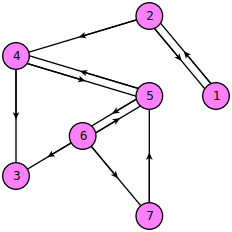
\includegraphics{seven_page_1}} 
\caption{A seven page internet}
\label{F:seven_page}
\end{center}
\end{figure}


To rank pages, we need to know how likely it is that a surfer will land on a given page. In our seven page example, a person can land on page 3 from page 4 with a probability of $\frac{1}{2}$ or from page 6 with a probability of $\frac{1}{3}$. If there is a link from a page we assume that the surfer leaves the page, and if there are no links from a page then the surfer stays on that page. We also assume that the surfer does not use the ``Back'' key. This information for our seven page internet example can be summarized in a \emph{transition matrix} $T$ whose $i,j$th entry is the probability that a surfer lands on page $i$ from page $j$.
\[T= \left[ \renewcommand{\arraystretch}{1.2} \begin{array}{ccccccc} 0&\frac{1}{2}&0&0&0&0&0 \\ 1&0&0&0&0&0&0 \\ 0&0&1&\frac{1}{2}&0&\frac{1}{3}&0 \\ 0&\frac{1}{2}&0&0&\frac{1}{2}&0&0 \\ 0&0&0&\frac{1}{2}&0&\frac{1}{3}&1 \\ 0&0&0&0&\frac{1}{2}&0&0 \\ 0&0&0&0&0&\frac{1}{3}&0 \end{array} \right].\]

Let us assume in our seven page internet that a user starts on page 6. That is, the probability that the user is initially on page 6 is 1, and so the probability that the user is on some other page is 0. This information can be encapsulated in a \emph{state vector}
\[\vx_0 = \left[ 0 \ 0 \ 0 \ 0 \ 0 \ 1 \ 0  \right]^{\tr}.\]
Since there are links from page 6 to pages 3, 5, and 7, there is a $\frac{1}{3}$ probability that the surfer will next move to one of these pages. That means that at the next step, the state vector $\vx_1$ for this user will be
\[\vx_1 = \left[ 0 \ 0 \ \frac{1}{3} \ 0 \ \frac{1}{3} \ 0 \ \frac{1}{3} \right]^{\tr}.\]
Note that
\[\vx_1 = T\vx_0.\]
As the user continues to surf the internet, the probabilities that the surfer is on a given page after the second, third, and fourth steps are given in the state vectors
\[\vx_2 = T\vx_1 = T^2 \vx_0, \ \ \vx_3 = T\vx_2 = T^3 \vx_0, \ \ \vx_4 = T\vx_3 = T^4 \vx_0.\]
In general, the probabilities that the surfer is on a given page after the $n$th step is given by the state vector
\[\vx_n = T \vx_{n-1} = T^n \vx_0.\]

This example illustrates the general nature of what is called a \emph{Markov process} (see Definition \ref{def:Markov}).  The two properties of the transition matrix $T$ make $T$ a special kind of matrix.

\begin{definition}  A \textbf{stochastic} matrix\index{stochastic matrix} is a matrix in which entries are nonnegative and the sum of the entries in every column is one.
\end{definition}

In a Markov process, each generation depends only on the preceding generation and there may be a limiting value as we let the process continue indefinitely. We can test to see if that happens for this Markov process defined by $T$ by doing some experimentation.


\begin{pactivity} \label{act:limit} Use appropriate technology to do the following. Choose several different initial state vectors $\vx_0$ and calculate the vectors in the sequence $\{T^n\vx_0\}$ for large values of $n$. (Note that, as state vectors, the entries of $\vx_0$ cannot be negative and the sum of the entries of $\vx_0$ must be $1$.) Explain the behavior of the sequence $\{\vx_n\}$ as $n$ gets large. Do you notice anything strange? What aspects of our seven page internet do you think explain this behavior? Clearly communicate all of the experimentation that you do. You may use the GeoGebra applet at \url{https://www.geogebra.org/m/b3dybnux}.  


\end{pactivity}



If there is a limit of the sequence $\{T^n\vx_0\}$ (in other words, if there is a vector $\vv$ such that $\vv = \ds \lim_{n \to \infty} T^n \vx_0$), we call this limit a \emph{steady-state} or \emph{equilibrium} vector. Such a steady-state vector has another important property. Since $T$ is independent of $n$ we have 
\begin{equation} \label{eq:Google_evector}
T \vv = T\left(\lim_{n \to \infty} T^n \vx_0 \right) = \lim_{n \to \infty} T^{n+1} \vx_0 = \vv.
\end{equation}


Equation (\ref{eq:Google_evector}) shows that a steady state vector $\vv$ is an eigenvector for $T$ with eigenvalue 1. We can interpret the steady-state vector for $T$ in an important way. Let $t_j$ be the fraction of time we spend on page $j$ and let $l_j$ be the number of links on page $j$. Then the fraction of the time that we end up on page $i$ coming from page $j$ is $\frac{t_j}{l_j}$. If we sum over all the pages linked to page $i$ we have that
\[t_i = \sum \frac{t_j}{l_j}.\]
Notice that this is essentially the same process we used to obtain $\vx_n$ from $\vx_{n-1}$, and so we can interpret the steady-state vector $\vv$ as telling us what fraction of a random web surfer's time was spent at each web page. If we assume that the time spent at a web page is a measure of its importance, then the steady-state vector tells us the relative importance of each web page. So this steady-state vector provides the page rankings for us. In other words,
\begin{quote}
The importance of a webpage may be measured by the relative size of the corresponding entry in the steady-state vector for an appropriately chosen Markov chain.
\end{quote}


\begin{pactivity} Show that the limiting vector you found in Project Activity \ref{act:limit} is an eigenvector of $T$ with eigenvalue 1.


\end{pactivity}


Project Activity \ref{act:limit} illustrates one problem with our seven page internet. The steady-state vector shows that page 3 is the only important page, but that hardly seems reasonable in the example since there are other pages that must have some importance. The problem is that page 3 is a ``dangling'' page and does not lead anywhere. Once a surfer reaches that page, they are  stuck there, overemphasizing its importance. So this dangling page acts like a sink, ultimately drawing all surfers to it. To adjust for dangling pages, we make the assumption that if a surfer reaches a dangling page (one with no links emanating from it), the surfer will jump to any page on the web with equal probability. So in our seven page example, once a surfer reaches page 3 the surfer will jump to any page on the web with probability $\frac{1}{7}$.

\begin{pactivity} \label{LQ:G2} ~
    \ba
    \item Determine the transition matrix for our seven page internet with this adjustment.

    \item Approximate the steady-state vector for this adjusted matrix so that the entries are accurate to four decimal places. Use any appropriate technology to row reduce matrices.
   

    \item According to this adjusted model, which web page is now the most important? Why? Does this seem reasonable? Why?


    \ea
\end{pactivity}

There is one more issue to address before we can consider ourselves ready to rank web pages. Consider the example of the five page internet shown in Figure \ref{F:five_page}.


\begin{figure}[h]
\begin{center}
\resizebox{!}{2.0in}{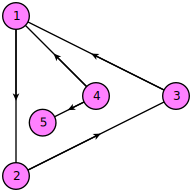
\includegraphics{five_page_1}} 
\caption{A five page internet}
\label{F:five_page}
\end{center}
\end{figure}


\begin{pactivity} \label{Q:no_limit} ~
    \ba
    \item Explain why
    \[\renewcommand{\arraystretch}{1.2} \left[ \begin{array}{ccccc} 0&0&1&\frac{1}{2}&\frac{1}{5} \\ 1&0&0&0&\frac{1}{5} \\ 0&1&0&0&\frac{1}{5} \\ 0&0&0&0&\frac{1}{5} \\ 0&0&0&\frac{1}{2}&\frac{1}{5} \end{array} \right].\]
is the transition matrix for this five page internet. (Keep in mind the adjustment we made for dangling pages.)

    \item Start with different initial state vectors $\vx_0$ and determine if there is a limit to the Markov chain. Explain. You may use the GeoGebra applet at \url{https://www.geogebra.org/m/b3dybnux}.  


    \ea
\end{pactivity}



Project Activity \ref{Q:no_limit} shows that it is possible to construct an internet so that the corresponding Markov chain does not have a limit, even after adjusting for dangling pages. This is a significant problem if we want to provide a relative ranking of all web pages regardless of where a surfer starts. To fix this problem we need to make one final adjustment to arrive at a type of transition matrix that always provides a limit for our Markov chain.

\begin{definition} A stochastic matrix is \textbf{regular}\index{stochastic matrix!regular} if its transition matrix $T$ has the property that for some power $k$, all the entries of $T^k$ are positive.
\end{definition}

Note that the transition matrix from Project Activity \ref{Q:no_limit} is not regular. Regular matrices have some especially nice properties, as the following theorem describes. We will not prove this theorem, but use it in the remainder of this project. The theorem shows that if we have a regular transition matrix, then there will a limit of the state vectors $\vx_n$, and that this limit has a very interesting property.

\begin{theorem} \label{thm:Google_1} Assume $n \geq 2$ and that $T$ is a regular $n \times n$ stochastic matrix.
\begin{enumerate}
\item $\ds \lim_{k \to \infty} T^k$ exists and is a stochastic matrix.
\item For any vector $\vx$,
\[\lim_{k \to \infty} T^k \vx = \vc\]
for the same vector $\vc$. 
\item The columns of $\ds \lim_{k \to \infty} T^k$ are the same vector $\vc$.
\item The vector $\vc$ is the unique eigenvector of $T$ whose entries sum to 1.
\item If $\lambda$ is an eigenvalue of $T$ not equal to 1, then $|\lambda| < 1$.
\end{enumerate}
\end{theorem}

 
Having a regular transition matrix $T$ ensures that there is always the same limit $\vv$ to the sequence $T^k \vx_0$ for any starting vector $\vx_0$. As mentioned before, the entries in $\vv = \ds \lim_{n \to \infty} T^n \vx_0$ can be interpreted as telling us what fraction of the random surfer's time was spent at each webpage. If we interpret the amount of time a surfer spends at a page as a measure of the page's importance, then this steady-state vector $\vv$ provides a ranking of the relative importance of each page in the web. This is the essence of Google's PageRank.

To make our final adjustment in the transition matrix to be sure that we obtain a regular matrix, we need to deal with the problems of ``loops'' in our internet. Loops, as illustrated in Project Activity \ref{Q:no_limit}, can act as sinks just like the dangling pages we saw earlier and condemn a user that enters such a loop to spend his/her time only on those pages in the loop. Quite boring! To account for this problem, we make a second adjustment.

Let $p$ be a number between 0 and 1 (Google supposedly uses $p=0.85$). Suppose a surfer is on page $i$. We assume with probability $p$ that the surfer will chose any link on page $i$ with equal probability. We make the additional assumption with probability $1-p$ that the surfer will select with equal probability any page on the web.

If $T$ is a transition matrix, incorporating the method we used to deal with dangling pages, then the adjusted transition matrix $G$ (the Google matrix) is
\[G = pT + (1-p)Q,\]
where $Q$ is the matrix all of whose entries are $\frac{1}{n}$, where $n$ is the number of pages in the internet ($n=7$ in our seven page example). Since all of the entries of $G$ are positive, $G$ is a regular stochastic matrix.



\begin{pactivity} Return to the seven page internet in Figure \ref{F:seven_page}.
    \ba
    \item Find the Google matrix $G$ for this internet.

    \item Approximate, to four decimal places, the steady-state vector for this internet. 

    \item What is the relative rank of each page in this internet, and approximately what percentage of time does a random user spend on each page.
    
    \ea
\end{pactivity}


We conclude with two observations. Consider the role of the parameter $p$ in our final adjustment. Notice that if $p=1$, then $G = T$ and we have the original hyperlink structure of the web. However, if $p=0$, then $G = \frac{1}{n} I_n$, where $I_n$ is the $n \times n$ identity matrix with $n$ as the number of pages in the web. In this case, every page is linked to every other page and a random surfer spends equal time on any page. Here we have lost all of the character of the linked structure of the web. Choosing $p$ close to 1 retains much of the original hyperlink structure of the web.

Finally, the matrices that model the web are HUGE, and so the methods we used in this project to approximate the steady-state vectors are not practical. There are many methods for approximating eigenvectors that are often used in these situations, some of which we discuss in a later section.






